Die Authentisierungszeit ist die Zeit zwischen erfolgreicher Eingabe des 
Benutzernamen und Passworts und der erfolgreichen Eingabe des TOTPs. Eingaben 
ungültiger TOTPs zählen nicht zu diesen Zeiten. Hat ein Proband sich angemeldet und 
musste sich aus technischen Gründen nochmal anmelden, so begann die Messung erneut.
\\\\
Die insgesamt 59 Messungen (ein Proband tätigte nur 5 anstatt 6 Anmeldungen) 
verteilen sich wie in Abb. \ref{fig: studie ergebnisse auth time dist} dargestellt. 
Das in Abb. \ref{fig: studie ergebnisse auth time boxplot} dargestellte Boxplot 
berücksichtigt die Ausreißer ($> 35~s$), zeigt sie aber nicht an.
\begin{figure}
    \begin{minipage}[t]{.48\textwidth}
        \centering
        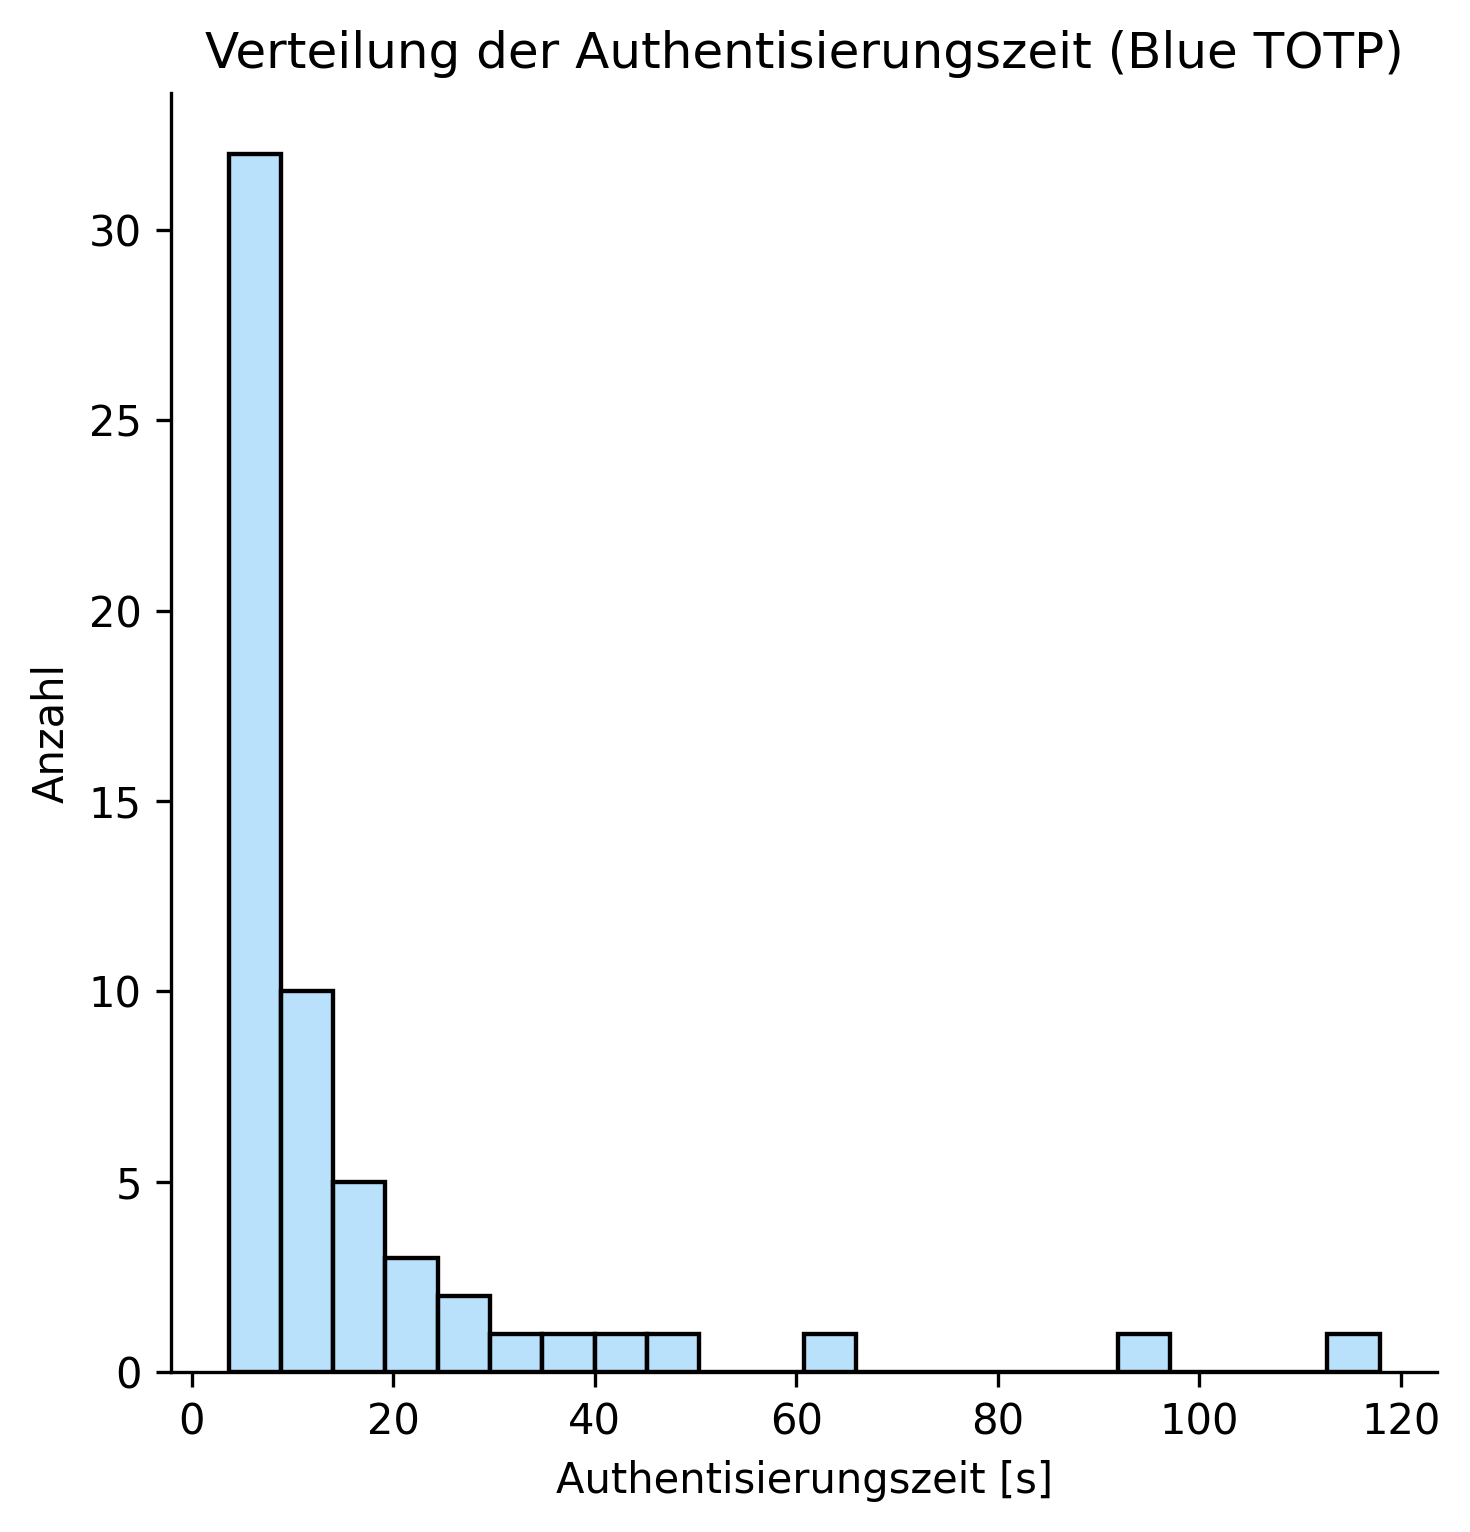
\includegraphics[width=1\linewidth]{data_processing/timings/results/distribution_of_data.png}
        \caption[Verteilung der Authentisierungszeiten (Blue TOTP)]{Verteilung der Authentisierungszeiten (Blue TOTP)}
        \label{fig: studie ergebnisse auth time dist}
    \end{minipage}
    \hfill
    \begin{minipage}[t]{.48\textwidth}
        \centering
        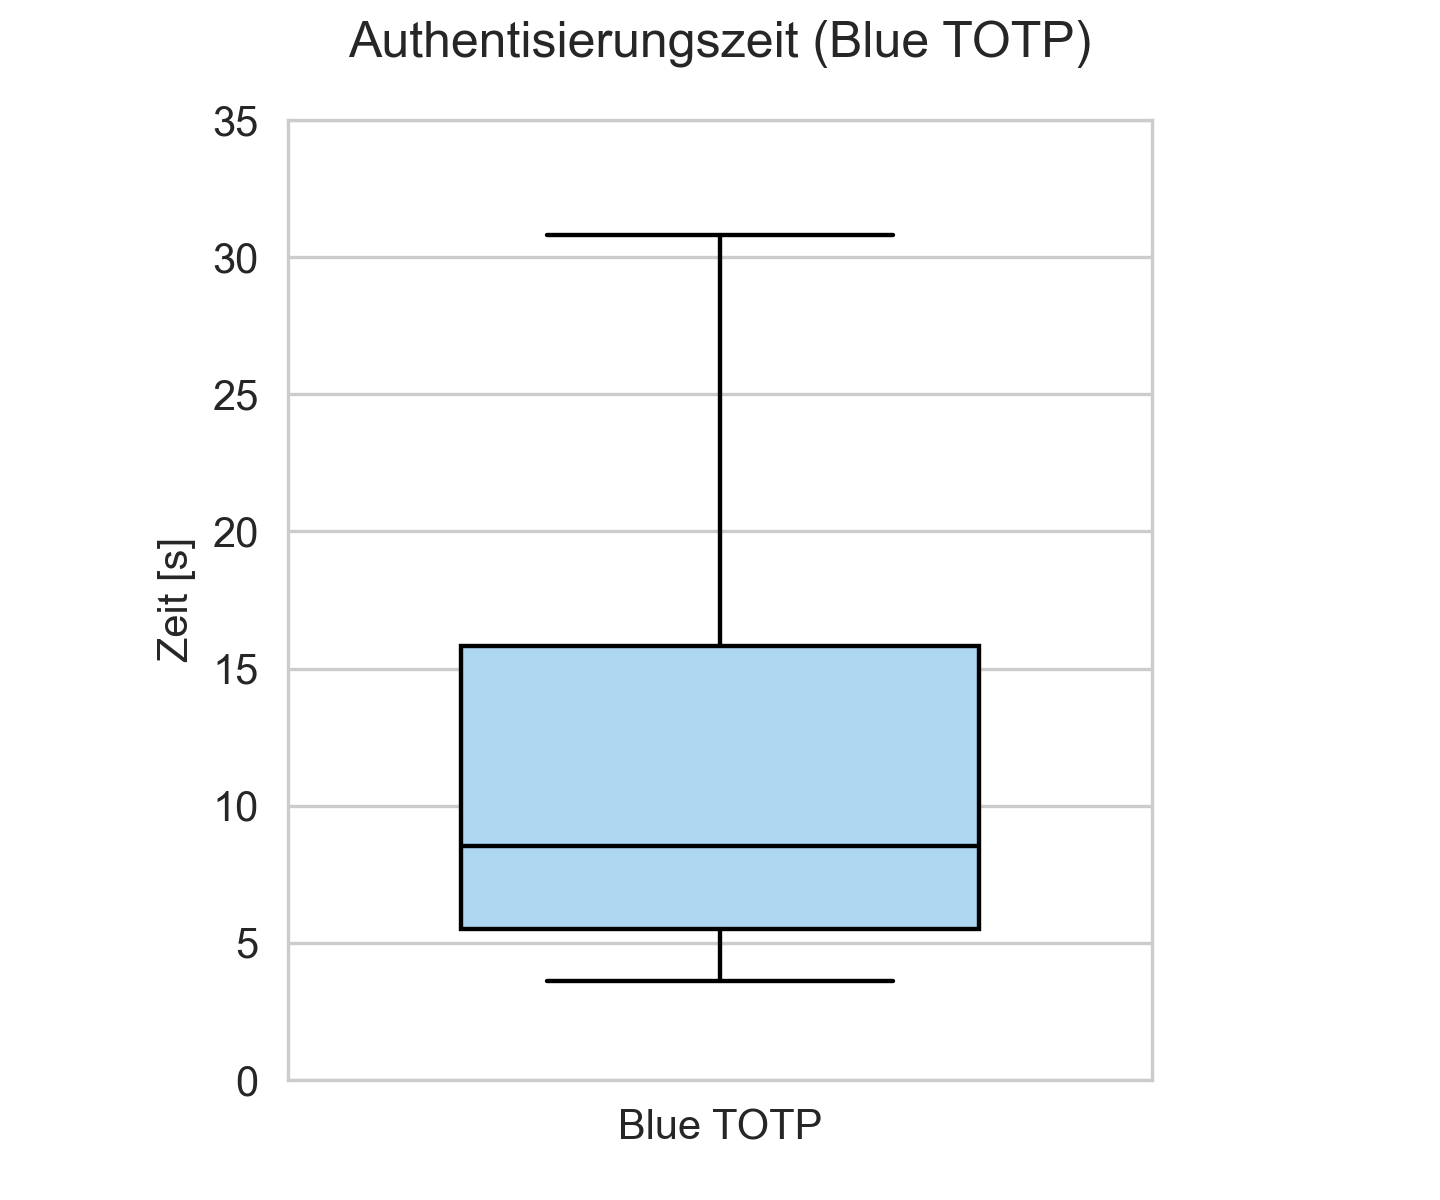
\includegraphics[width=1.2\linewidth]{data_processing/timings/results/totp_timings_boxplot.png}
        \caption[Authentisierungszeit von Blue TOTP]{Authentisierungszeit von Blue TOTP}
        \label{fig: studie ergebnisse auth time boxplot}
    \end{minipage}
\end{figure}
Über 30 der 59 Werte liegen unter $10~s$. Die kürzeste Messung beträgt $3{,}6~s$. Es gibt einige Ausreißer wie die drei über 
$60~s$. Es ist unklar, wieso die Probanden bei diesen Messungen übermäßig Zeit 
benötigten. Alle Messungen bilden einen Median von $8{,}5~s$ und einen Mittelwert von 
$15{,}9~s$. Bereinigt man die Daten nach dem Verfahren des $1{,}5$-fachen 
Interquartilsabstands (Entfernen aller Werte $> 31{,}3~s$), erhält man einen 
Mittelwert von $10,1~s$ (siehe Anhang \ref{anh: studie ergebnisse auth} Tab. \ref{tab: 
studie ergebnisse auth time}).
\\\\
Die Authentisierungszeiten pro Tag der Nutzungsphase sind in Abb. \ref{fig: studie 
ergebnisse auth time days} dargestellt. Das Diagramm zeigt nur den Wertebereich bis 
$40~s$, um die dichten Datenpunkte besser zu unterscheiden.
\begin{figure}
    \centering
    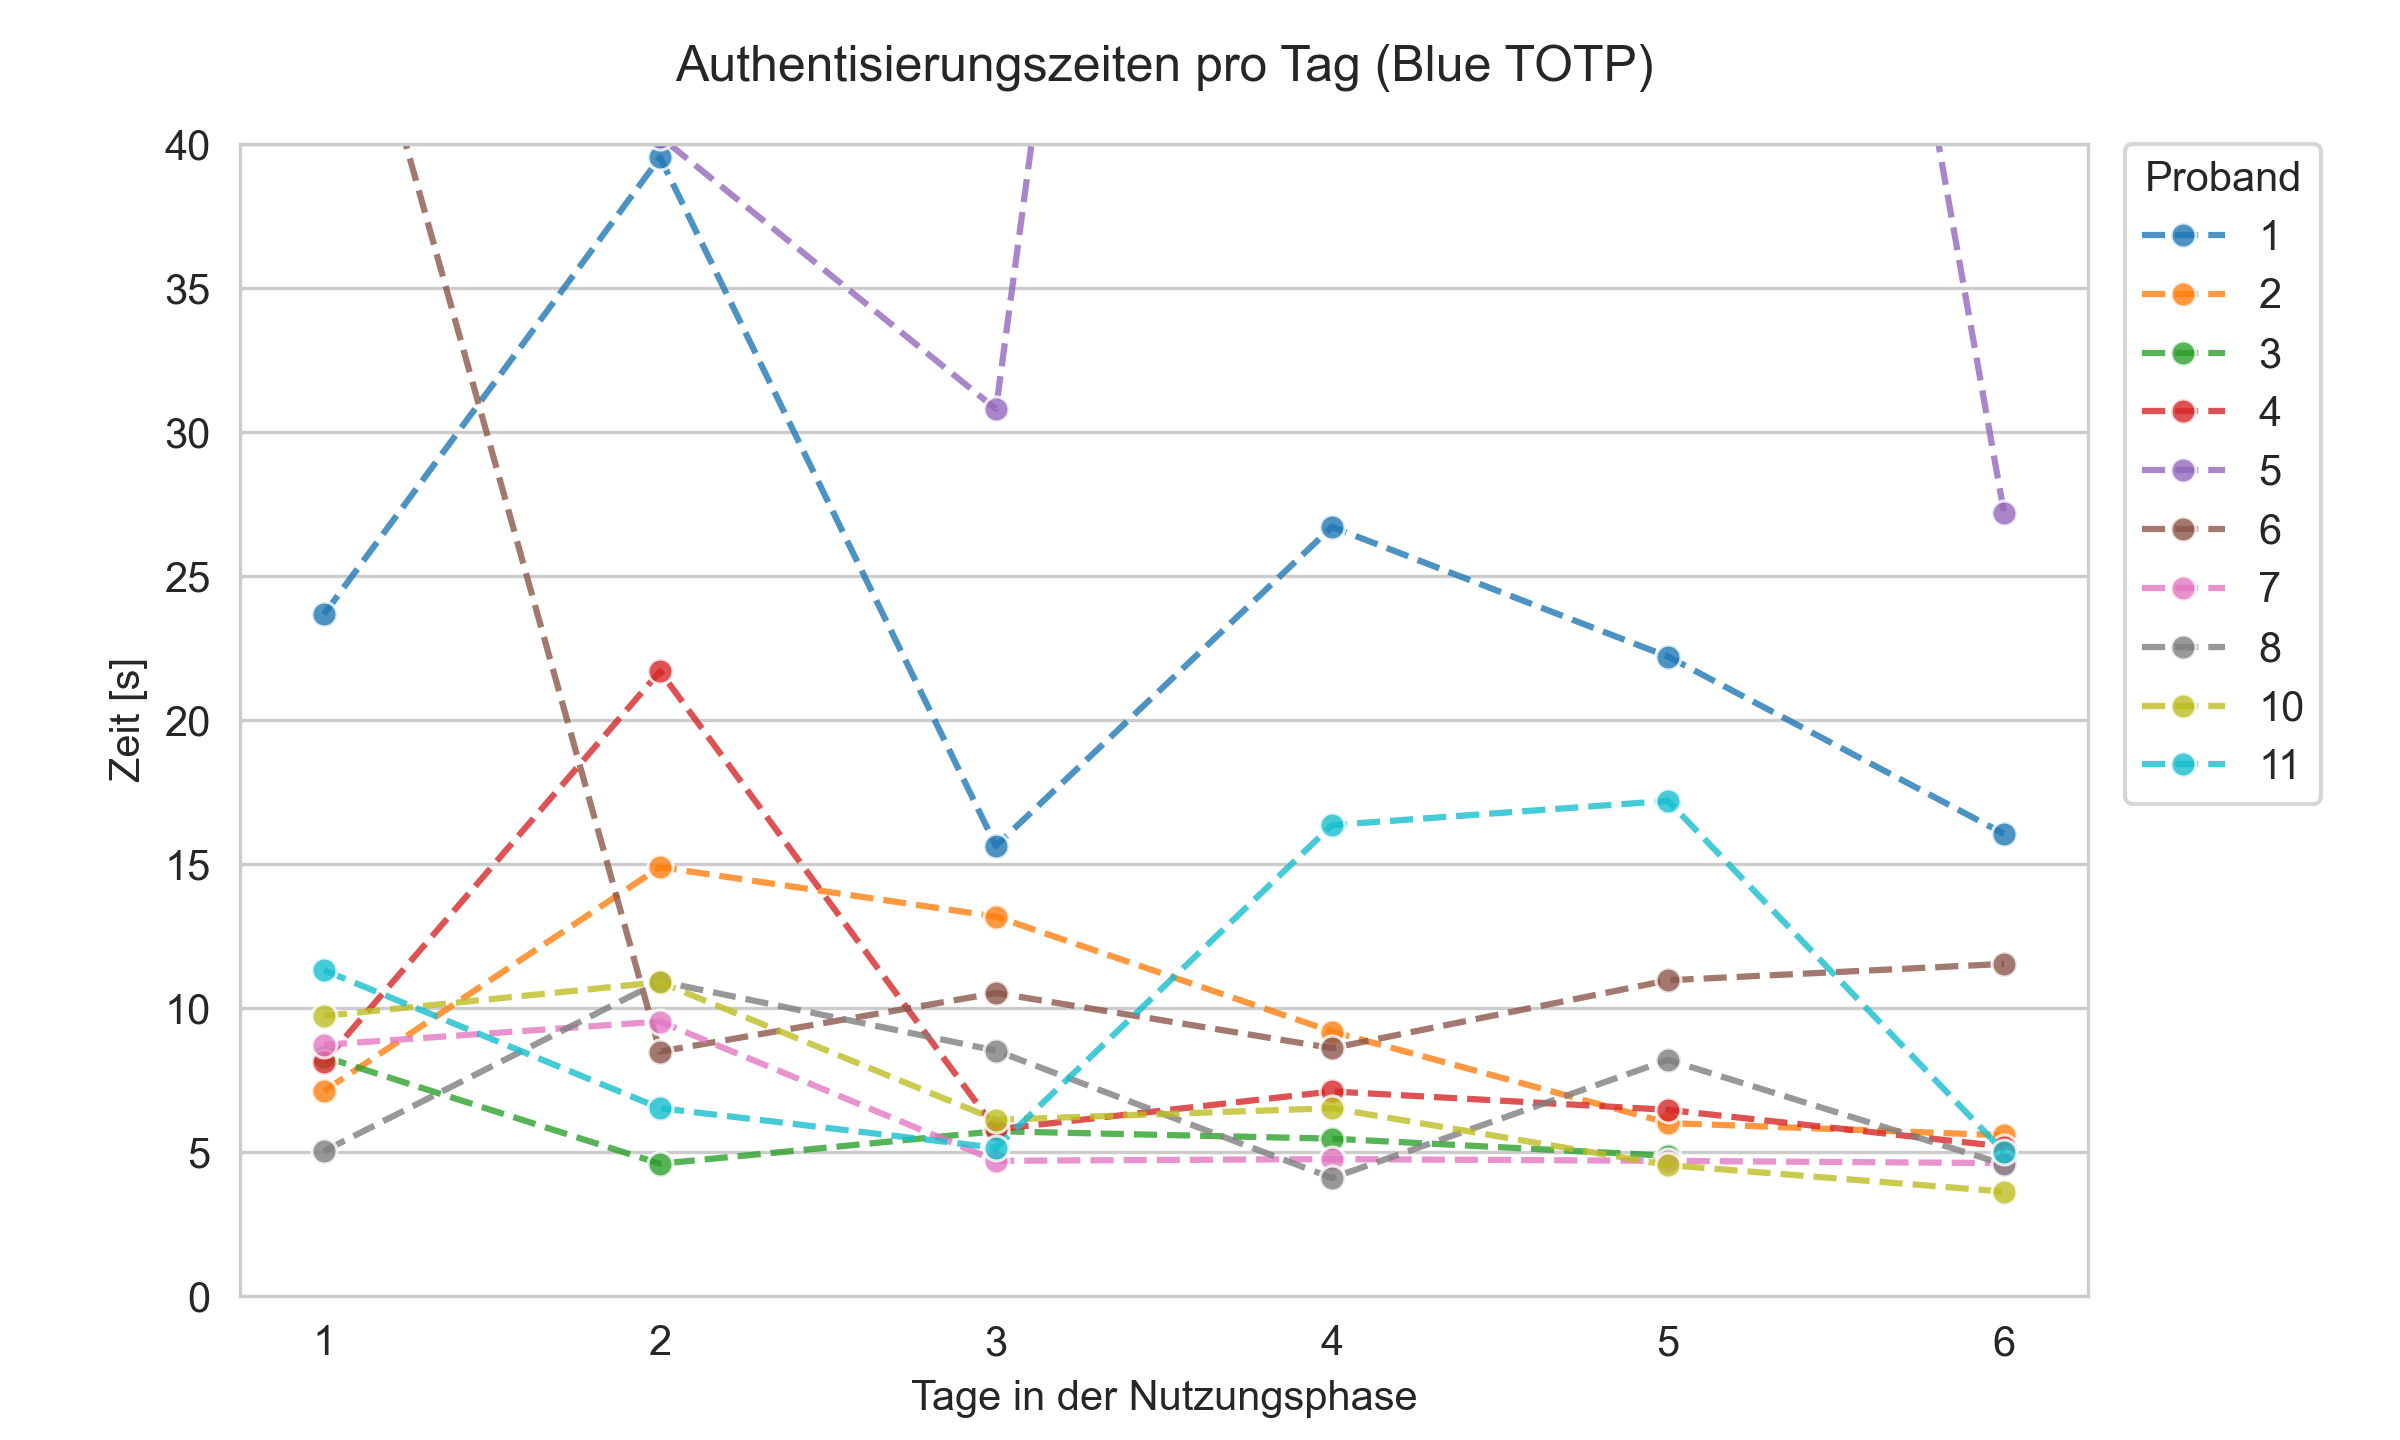
\includegraphics[width=0.85\linewidth]{data_processing/timings/results/totp_timings_lineplot.png}
    \caption[Authentisierungszeiten pro Tag in der Nutzungsphase (Blue TOTP)]{Authentisierungszeiten pro Tag in der Nutzungsphase (Blue TOTP)}
    \label{fig: studie ergebnisse auth time days}
\end{figure}
Die Verläufe der einzelnen Linien lässt im Gesamtbild keine klare Tendenz erkennen, 
ob die Probanden über die Dauer der Nutzungsphase die Authentisierung immer schneller 
durchführten. Lässt man die Probanden 1,5 und 6 außen vor, erkennt man, dass die 
verbleibenden 7 Probanden bis auf einzelne Ausnahmen immer weniger als $15~s$ 
benötigt haben. Auch ist erkennbar, dass diese 7 Probanden am letzten Tag nur ca. 
$5~s$ benötigten und im Vergleich zum ersten Tag schneller waren. Betrachtet man die 
Medianwerte aller Messungen pro Tag in der Nutzerstudie, wie in Tab. \ref{tab: studie 
ergebnisse auth time median days} dargestellt, dann lässt sich dahingehend auch ein 
Trend erkennen.
\begin{table}
    \centering
    \begin{center}
    \begin{tabular}{| l | c | c | c | c | c | c |}
        \hline
        \textbf{Tag} & $1$ & $2$ & $3$ & $4$ & $5$ & $6$ \\
        \hline
        \textbf{Median} & $9{,}2~s$ & $10{,}9~s$ & $7{,}3~s$ & $7{,}9~s$ & $7{,}3~s$ & $5{,}2~s$ \\
        \hline
    \end{tabular}
    \end{center}
    \caption[Median der Authentisierungszeit pro Tag in der Nutzungsphase]{Median der Authentisierungszeit pro Tag in der Nutzungsphase}
    \label{tab: studie ergebnisse auth time median days}
\end{table}
Die Analyse mithilfe der Repeated Measures Correlation zwischen den Tagen der 
Nutzungsphase und den Authentisierungszeiten pro Proband ergab einen 
Korrelationskoeffizienten von $r = -0{,}1634$ und keine statistische Signifikanz, da 
$p > 0{,}05$ (siehe Anhang \ref{anh: studie ergebnisse auth} Tab. \ref{tab: studie 
ergebnisse auth time rmcorr}). Dennoch ist die negative Richtung der Korrelation 
zwischen Tag der Nutzungsphase und Authentisierungszeit deutlich.
\\\\
Bei dem Versuch, die tägliche Aufgabe im Webservice zu lösen, kam es bei 23 der 
insgesamt 59 Sitzungen vor, dass die Probanden Benutzername und Passwort mindestens 
einmal erneut eingeben mussten, wahrscheinlich weil sie die App und Extension 
nicht vor der Eingabe von Benutzername und Passwort miteinander verbunden hatten. In diesem Fall wurde das TOTP nicht automatisch von der 
App an die Extension übertragen. Insgesamt gab es 36 fehlgeschlagene 
Loginversuche.